\subsection{Mehrphasensysteme 1}
\Aufgabe{
    Gegeben ist ein unsymmetrisches System mit folgenden Spannungen:
   
    $\underline{U}_\mathrm{L1}=230 V$, $\underline{U}_\mathrm{L2}=460 V\cdot e^{-j45^\circ}$, $\underline{U}_\mathrm{L1}=345 V\cdot e^{j120^\circ}$
 
    \begin{itemize}
        \item [a)] Zeichen Sie das Zeigerdiagramm des Originalsystems!
        \item [b)] Stellen Sie die Zerlegungsgleichungen für die Spannungen auf!
        \item [c)] Berechnen Sie die Spannungen der transformierten Systeme!
        \item [d)] Zeichen Sie die Zeigerdiagramme der transformierten Systeme!
    \end{itemize}
}


\Loesung{
	\begin{itemize}
		
	\item[\bf a)]
	
        Zeigerdiagramm des Originalsystems: \\
        \begin{figure}[H]
            \centering
            \resizebox{0.6\textwidth}{!}{%
                    \begin{tikzpicture}
                        \draw [->] (0, 0) -- (2, 0);
                        \draw [->] (0, 0) -- (2.83, -2.83);
                        \draw [->] (0, 0) -- (-1.5, 2.6);
                    
                        \draw (1.8, 0.3) node {$\underline{U}_{\mathrm{L1}}{=}230V$};
                        \draw (0.8, 1.4) node {$\underline{U}_{\mathrm{L3}}{=}345V\cdot e^{j120^{\circ}}$};
                        \draw (4, -2) node {$\underline{U}_{\mathrm{L2}}{=}460V\cdot e^{-j45^{\circ}}$};
                    
            \end{tikzpicture}%
            }
        \end{figure}
        
    \item[\bf b)]
        \begin{eqa}
            \underline{U}_{\mathrm{L1}}&=230 V=\underline{U}_{0}+\underline{U}_{1}+\underline{U}_{2} \notag \\
            \underline{U}_{\mathrm{L2}}&=460 V\cdot e^{-j45^\circ}=\underline{U}_{0}+\underline{a}^2\cdot \underline{U}_{1}+\underline{a}\cdot\underline{U}_{2} \notag \\
            \underline{U}_{\mathrm{L3}}&=345 V\cdot e^{j120^\circ}=\underline{U}_{0}+\underline{a}\cdot\underline{U}_{1}+\underline{a}^2\cdot\underline{U}_{2} \notag
        \end{eqa}
        
    \item[\bf c)]
        Für das Nullsystem:
        
        \begin{eqa}
            \underline{U}_0&=\frac{1}{3}\cdot(\underline{U}_{\mathrm{L1}}+\underline{U}_{\mathrm{L2}}+\underline{U}_{\mathrm{L3}}) \notag \\
            &=\frac{1}{3}\cdot(230 V+460 V\cdot e^{-j45^\circ}+345 V\cdot e^{j120^\circ}) \notag \\
            &=\frac{1}{3}\cdot(230V+325,27V-j325,27V-172,5V+298,78V) \notag \\
            &=127,59V-j8,83=127,9\cdot e^{-j3,56^\circ} \notag
        \end{eqa}
        
        Für das Mitsystem:
        
        \begin{eqa}
            \underline{U}_{1}&=\frac{1}{3}\cdot(\underline{U}_{\mathrm{L1}}+\underline{a}\cdot\underline{U}_{\mathrm{L2}}+\underline{a}^2\cdot\underline{U}_{\mathrm{L3}}) \notag \\
            &=\frac{1}{3}\cdot(230V+(-\frac{1}{2}+j\frac{\sqrt{3}}{2})\cdot(325,27V-j325,7V)+(-\frac{1}{2}-j\frac{\sqrt{3}}{2})\cdot(-172,5V+298,78V)) \notag \\
            &=\frac{1}{3}\cdot(230V+119,42V+j444,54V+345V) \notag \\
            &=231,48V+j148,18V=274,84\cdot e^{j32,63^\circ} \notag
        \end{eqa}
        
        
        Für das Gegensystem:
        
        \begin{eqa}
            \underline{U}_{2}&=\frac{1}{3}\cdot(\underline{U}_{\mathrm{L1}}+\underline{a}^2\cdot\underline{U}_{\mathrm{L2}}+\underline{a}\cdot\underline{U}_{\mathrm{L3}}) \notag \\
            &=\frac{1}{3}\cdot(230V+(-\frac{1}{2}-j\frac{\sqrt{3}}{2})\cdot(325,27V-j325,7V)+(-\frac{1}{2}+j\frac{\sqrt{3}}{2})\cdot(-172,5V+298,78V)) \notag \\
            &=\frac{1}{3}\cdot(230V+(-444,33V-j119,16V)+(-172,5V-298,78V)) \notag \\
            &=-128,95V-j139,28V=189,8\cdot e^{j132,79^\circ} \notag
        \end{eqa}
        
    \item[\bf d)]
    
        Zeigerdiagramme der transformierten Systeme: \\
        \begin{figure}[H]
            \centering
            \resizebox{0.8\textwidth}{!}{
            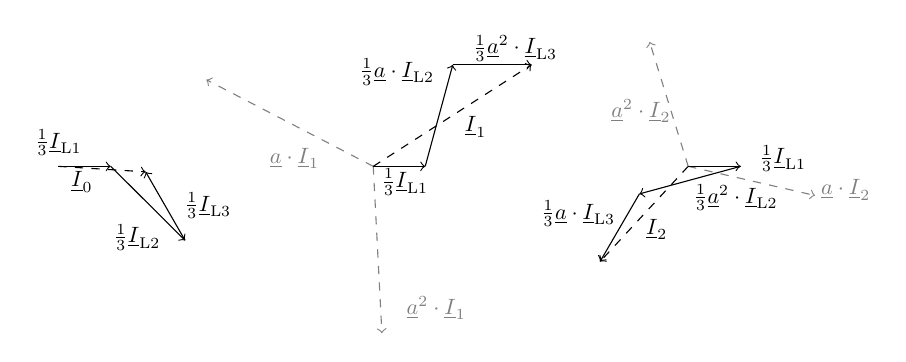
\begin{tikzpicture}
                \draw [->] [dashed] (0, -6) -- (2.01, -4.71);
                \draw [->, gray] [dashed] (0, -6) -- (-2.12, -4.9);
                \draw [->, gray] [dashed] (0, -6) -- (0.11, -8.12);
                \draw [->] (0, -6) -- (0.66, -6);
                \draw [->] (0.66, -6) -- (1.01, -4.71);
                \draw [->] (1.01, -4.71) -- (2.01, -4.71);
            
                \draw (1.3, -5.5) node [scale=0.8] {$\underline{I}_{\mathrm{1}}$};
                \draw (-1, -5.9) node [scale=0.8, gray] {$\underline{a}\cdot\underline{I}_{\mathrm{1}}$};
                \draw (0.8, -7.8) node [scale=0.8, gray] {$\underline{a}^2\cdot\underline{I}_{\mathrm{1}}$};
                \draw (0.4, -6.2) node [scale=0.8] {$\frac{1}{3}\underline{I}_{\mathrm{L1}}$};
                \draw (1.8, -4.5) node [scale=0.8] {$\frac{1}{3}\underline{a}^2\cdot\underline{I}_{\mathrm{L3}}$};
                \draw (0.3, -4.8) node [scale=0.8] {$\frac{1}{3}\underline{a}\cdot\underline{I}_{\mathrm{L2}}$};
            
                \draw [->] [dashed] (4, -6) -- (2.88, -7.21);
                \draw [->, gray] [dashed] (4, -6) -- (5.61, -6.37);
                \draw [->, gray] [dashed] (4, -6) -- (3.51, -4.42);
                \draw [->] (4, -6) -- (4.666, -6);
                \draw [->] (4.666, -6) -- (3.38, -6.35);
                \draw [->] (3.38, -6.35) -- (2.88, -7.21);
            
                \draw (3.6, -6.8) node [scale=0.8] {$\underline{I}_{\mathrm{2}}$};
                \draw (6, -6.3) node [scale=0.8, gray] {$\underline{a}\cdot\underline{I}_{\mathrm{2}}$};
                \draw (3.4, -5.3) node [scale=0.8, gray] {$\underline{a}^2\cdot\underline{I}_{\mathrm{2}}$};
                \draw (5.2, -5.9) node [scale=0.8] {$\frac{1}{3}\underline{I}_{\mathrm{L1}}$};
                \draw (4.6, -6.4) node [scale=0.8] {$\frac{1}{3}\underline{a}^2\cdot\underline{I}_{\mathrm{L2}}$};
                \draw (2.6, -6.6) node [scale=0.8] {$\frac{1}{3}\underline{a}\cdot\underline{I}_{\mathrm{L3}}$};
            
                \draw [->] [dashed] (-4, -6) -- (-2.89, -6.07);
                \draw [->] (-4, -6) -- (-3.334, -6);
                \draw [->] (-3.334, -6) -- (-2.39, -6.94);
                \draw [->] (-2.39, -6.94) -- (-2.89, -6.07);
            
                \draw (-3.7, -6.2) node [scale=0.8] {$\underline{I}_{\mathrm{0}}$};
                \draw (-4, -5.7) node [scale=0.8] {$\frac{1}{3}\underline{I}_{\mathrm{L1}}$};
                \draw (-3, -6.9) node [scale=0.8] {$\frac{1}{3}\underline{I}_{\mathrm{L2}}$};
                \draw (-2.1, -6.5) node [scale=0.8] {$\frac{1}{3}\underline{I}_{\mathrm{L3}}$};
            \end{tikzpicture}
            }
        \end{figure}
        
        Anmerkung: Das Erstellen der Zeigerdiagramme ist ein guter Weg um die errechneten Ergebnisse aus 3. zu überprüfen.
        Die Wege der Zeiger, die aus dem Originalsystem genommen werden, müssen da enden, wo auch der Zeiger des transformierten Systems hinführt.
        Stimmen die Endpunkte nicht überein, wurde in einer der Rechnungen ein Fehler gemacht.

        \end{itemize}
}